\begin{frame}[plain]
    \begin{center}
        \vspace{48pt}
        {\huge\bf アナログ入力装置}
    \end{center}
\end{frame}

\begin{frame}
    \frametitle{感圧センサ}
    \begin{center}
        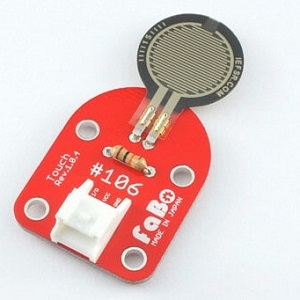
\includegraphics[width=0.4\textwidth]{images/chap05/text05-img021.jpg}
        \begin{itemize}
            \item 加えた力の大きさの変化を測ることができる
            \item 力を加えると値が小さくなる
            \item 0〜1023の間を値をとる
        \end{itemize}
    \end{center}
\end{frame}

\begin{frame}
    \frametitle{ボリューム}
    \begin{center}
        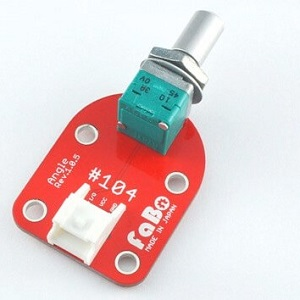
\includegraphics[width=0.4\textwidth]{images/chap05/text05-img022.jpg}
        \begin{itemize}
            \item シャフト(じく)をひねると値の大きさを変えることができる
            \item 0〜1023の間の値をとる
            \item 左に回しきったときは変化が小さくて、右に回していくほどに変化が大きくなる(Aカーブ)
        \end{itemize}
    \end{center}
\end{frame}

\begin{frame}
    \frametitle{距離(きょり)センサ}
    \begin{center}
        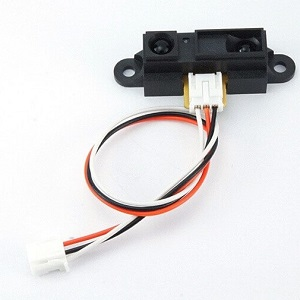
\includegraphics[width=0.4\textwidth]{images/chap05/text05-img023.jpg}
        \begin{itemize}
            \item 距離を測ることができる
            \item 10〜80cmの距離を測ることができる
            \item ただし値は0〜1023だから、値を距離に変換しないといけない
        \end{itemize}
    \end{center}
\end{frame}

\begin{frame}
    \frametitle{照度(しょうど)センサ}
    \begin{center}
        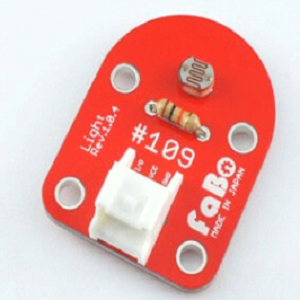
\includegraphics[width=0.4\textwidth]{images/chap05/text05-img024.png}
        \begin{itemize}
            \item 明るさの変化を測ることができる
            \item 暗いと値が大きく、明るいと値が小さくなる
        \end{itemize}
    \end{center}
\end{frame}

\begin{frame}
    \frametitle{センサーをピンにつけてみよう}
    \begin{center}
        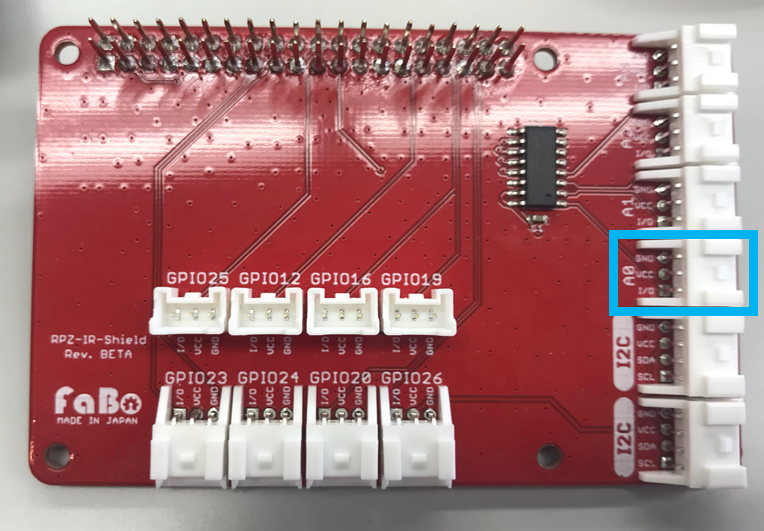
\includegraphics[width=0.8\textwidth]{images/chap05/text05-img030.png}
        \begin{itemize}
            \item A0とアナログ入力装置をつなげてみよう
            \item HSPでanain.hspを動かしてみよう
        \end{itemize}
    \end{center}
\end{frame}

\begin{frame}[fragile]
    \frametitle{アナログ入力を使ったサンプル(anain.hsp)}
\begin{lstlisting}
#include "hsp3dish.as"
#include "rpz-gpio.as"

spiopen 0

*main
	data = spiget(0,0)
	res = "結果 : "+data+"\n"

	redraw 0
	pos 20,20
	font "",30
	mes res
	redraw 1

	wait 10
	goto *main

spiclose 0
\end{lstlisting}
\end{frame}

\begin{frame}[fragile]
    \begin{itemize}
        \item 教科書17ページ 問題5-7
        \begin{itemize}
            \item 4問
        \end{itemize}
    \end{itemize}
\end{frame}
